
%%%%%%%%%%%%%%%%%%%%%%% file typeinst.tex %%%%%%%%%%%%%%%%%%%%%%%%%
%
% This is the LaTeX source for the instructions to authors using
% the LaTeX document class 'llncs.cls' for contributions to
% the Lecture Notes in Computer Sciences series.
% http://www.springer.com/lncs       Springer Heidelberg 2006/05/04
%
% It may be used as a template for your own input - copy it
% to a new file with a new name and use it as the basis
% for your article.
%
% NB: the document class 'llncs' has its own and detailed documentation, see
% ftp://ftp.springer.de/data/pubftp/pub/tex/latex/llncs/latex2e/llncsdoc.pdf
%
%%%%%%%%%%%%%%%%%%%%%%%%%%%%%%%%%%%%%%%%%%%%%%%%%%%%%%%%%%%%%%%%%%%


\documentclass[runningheads,a4paper]{llncs}

\usepackage{amssymb}
\setcounter{tocdepth}{3}
\usepackage{graphicx,caption}
\usepackage{amsmath}
\usepackage{amsfonts} 
\usepackage{tikz}
\newcommand*\circled[1]{\tikz[baseline=(char.base)]{
            \node[shape=circle,draw,inner sep=0.5pt] (char) {#1};}}
\newcommand{\vect}[1]{\mbox{\boldmath${#1}$}}%$
\DeclareMathOperator*{\argmin}{arg\,min}

\usepackage{url}
\urldef{\mailsa}\path|{meguenani,padois,dasilva,hoarau,bidaud}@isir.upmc.fr|    
\newcommand{\keywords}[1]{\par\addvspace\baselineskip
\noindent\keywordname\enspace\ignorespaces#1}




\begin{document}
\mainmatter  % start of an individual contribution

\title{Energy based control for safe human-robot physical interaction}

\author{Anis Meguenani
\and Vincent Padois\and Jimmy Da Silva \and Antoine Hoarau \and Philippe Bidaud}

\authorrunning{Anis Meguenani
\and Vincent Padois\and Philippe Bidaud}


\institute{Sorbonne Universit\'{e}s, UPMC Univ Paris 06, CNRS UMR 7222, Institut des Syst\`{e}mes Intelligents et de Robotique, F-75005, Paris, France\\
\mailsa\\
\mailsb\\
\mailsc}

\toctitle{Safety and constraints compatibility}

\maketitle




\begin{abstract}
In this paper, we propose physically meaningful energy related safety indicators for robots sharing their workspace with humans. Based on these indicators, safety criteria are introduced as constraints in the control algorithm.
The first constraint is placed on the kinetic energy of the robotic system to limit the amount of dissipated energy in case of collision. This constraint depends on the distance between the robot and the human operator. The distance is computed with a point cloud based algorithm acquired using a set of depth sensors (Kinects). The second constraint is on the amount of potential energy that is allowed to be generated within the human-robot system during physical contact. It is used to modulate the contact forces. The control algorithm is formulated as an optimization problem and computes every time step the actuation torques for a KUKA LWR4 manipulator given some task to be performed, the introduced constraints and the physical limitations of the system to respect. The overall framework allows a human operator to safely enter the robot's workspace and physically interact with it.  

\keywords{Safety, Human-robot interaction, Constraints compatibility, Energy, QP.}




%%%%%%%%%%%%%%%%%%%%%%%%%%%%%%%%%%%%%%%%%%%%%%%%%%%%%%%%%
%%%%%%%%%%%%%%%%%%%%%%%%%%%%%%%%%%%%%%%%%%%%%%%%%%%%%%%%%
                     %INTRODUCTION%
%%%%%%%%%%%%%%%%%%%%%%%%%%%%%%%%%%%%%%%%%%%%%%%%%%%%%%%%%
%%%%%%%%%%%%%%%%%%%%%%%%%%%%%%%%%%%%%%%%%%%%%%%%%%%%%%%%%
\section{Introduction}
\vspace{-2 mm}
Domains of application for robots are evolving from a purely structured industrial context to the human world as intervention machines and assistants to aid a person in the completion of a manual task. Safety is therefore of most importance. This has a direct impact on the formulation of the control problem that must be completely reconsidered. 
When industrial robots are aimed for tasks that are relatively simple e.g. pick and place manipulation, repetitive, within perfectly known static and protected environments; Intervention and service robotic systems are confronted to more challenging scenarios : unknown, constrained and dynamic environments and possible deliberate/undeliberate interactions with humans. 

To ensure safe human-robot interactions, several approaches have been explored in the robotics literature. At the hardware level, the mechanical design have been optimized by including torque sensing at the joint level. This provides a way to actively control the impedance of the robot. The Kuka-DLR lightweight robot \cite{bischoff2010kuka} has been specifically designed for these purposes.

On the software level, different control approaches using intrinsic
and extrinsic force/torque sensors have been developed to handle safety during pre and post impact/contact phases \cite{ebert2002safe}. Haddadin in \cite{haddadin2008collision} and De Luca in \cite{de2006collision} present different strategies to reduce the effect of non deliberate impacts. A collision detection parameter based on the sensed external torque is introduced and used to scale down the link inertia obtaining a  ``lighter" robot that ``flees" from the collision area. Heizmann and Zelinsky in \cite{heinzmann2003quantitative} propose a safety criterion based on the \textit{potential impact force} to filter the control torque of the system.

\begin{figure}
    \centering
    \captionsetup{width=.81\linewidth}
	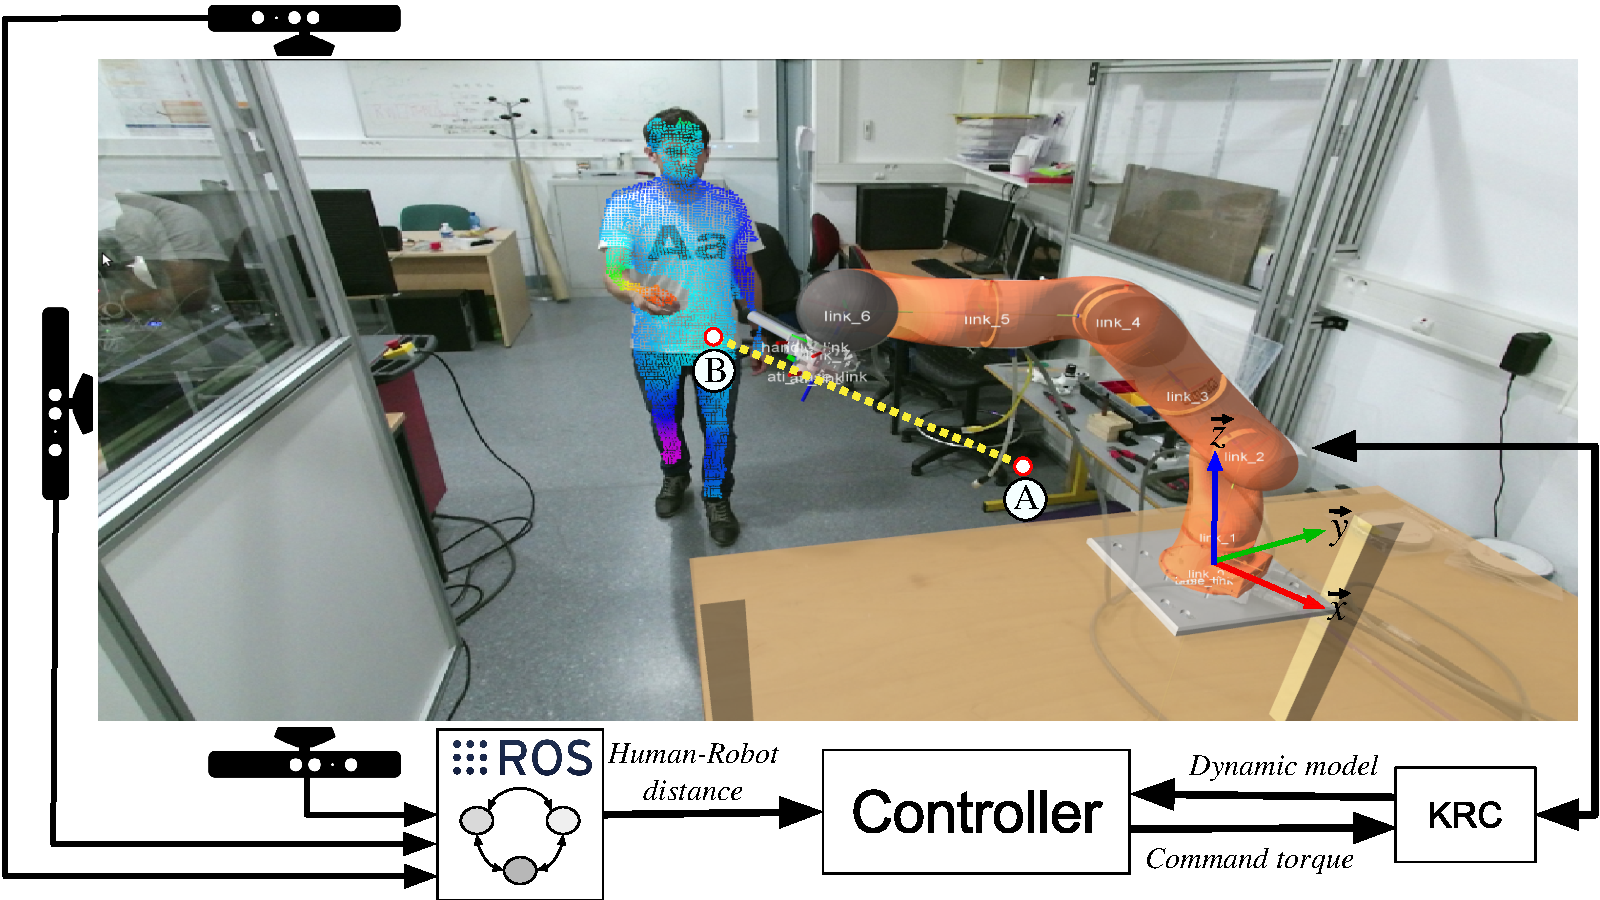
\includegraphics[width=.84\linewidth]{figures/HR_INT_HW_STRUCT}
    \caption{View of a user sharing its workspace with a KUKA LWR4 manipulator; with the experimental setup used to detect the human operator and control the robotic system.}
    \label{fig:HR_INT_HW_STRUCT}
\end{figure}

During human-robot interaction, the degree of danger towards the person is mainly caused by two parameters : the impact force created at the collision instant and the contact forces existing after the establishment of physical contact. 
The most generic way to include and express these parameters is to use an energetic formulation. Indeed, energy is a universal entity that can describe all the physical phenomena occurring during human-robot interaction. 
Energy has already been discussed in \cite{haddadin2008collision} and \cite{haddadin2012truly} as a good representation of the risk of injury. It is used in this work to synthesize indicators whose value is related to both impact and contact forces and that can be expressed using the control input. Safety criteria, namely a bound on the maximum value of the safety indicators, is then derived. Kinetic and potential energy based criteria are used to constrain the dynamic behaviour of a KUKA LWR4 serial robot during the interaction with a human operator. 
The present paper is the continuation of our previously published work \cite{meguenani2015control}. It is organised as follows. In section~II, the proposed safety indicators and associated safety criteria are formulated. In Section~III, the controller is derived : task's related objectives are formulated and the expression of the inequality constraints acting on the system is provided. In Section~IV, an experimental scenario is introduced based on which the possibilities offered by the proposed controller are illustrated and discussed. Finally, Section~V summarizes the contribution and provides an overview of the future work.


%%%%%%%%%%%%%%%%%%%%%%%%%%%%%%%%%%%%%%%%%%%%%%%%%%%%%%%%%
%%%%%%%%%%%%%%%%%%%%%%%%%%%%%%%%%%%%%%%%%%%%%%%%%%%%%%%%%
                  %SAFETY INDICARTORS%
%%%%%%%%%%%%%%%%%%%%%%%%%%%%%%%%%%%%%%%%%%%%%%%%%%%%%%%%%
%%%%%%%%%%%%%%%%%%%%%%%%%%%%%%%%%%%%%%%%%%%%%%%%%%%%%%%%%
\section{Interaction forces and the safety indicators}
\vspace{-2 mm}
%%%%%%%%%%%%%%%%%%%%%%%%%%%%%%%%%%%%%%%%%%%%%%%%%%%%%%%%%
                     %IMPACT FORCE%
%%%%%%%%%%%%%%%%%%%%%%%%%%%%%%%%%%%%%%%%%%%%%%%%%%%%%%%%%
\subsection{Impact force}
The generated impact force at collision can be written as a function of the dissipated energy and the shock absorption distance:
\begin{equation}
\int_u F_{impact} du = E_{dissipated} = E_{c}^{hum} + E_{c}^{rob},
\label{eq:Energydissipationmodel}
\end{equation}

$ F_{impact} $ is the generated impact force during the collision, $u$ the shock absorption distance and $E_{dissipated}$ the dissipated energy which is equal to the sum of the kinetic energy $E_{c}$ of both the human operator and the robot. At a given time, very few assumptions can be made on the state of energy of the human operator. As a consequence, the retained safety indicator $S_c$ is robot-centred. $E_{c}^{rob}$ is directly related to the impact force and can be expressed using the actuation torque. It is therefore to be considered for the formulation of the first safety indicator : 
\begin{equation}
\begin{split}
 S_c = E_{C}^{i,j} = \frac{1}{2}  m(\vect{q})_{i,j}^{eq} v_{i,j}^2
\end{split} 
\end{equation}
With $1/m(\vect{q})_{i,j}^{eq}  = J(\vect{q})_{C}^{i,j} M(\vect{q})^{-1} J(\vect{q})_{C}^{{i,j}^T}$. $m(\vect{q})_{i,j}^{eq}$ is the equivalent mass of the robot segment $i$ in the direction of obstacle $j$ expressed in the cartesian space. $M(\vect{q})$ is the joint space inertia matrix of the robot and $\vect{q}$ its joint space configuration. $v_{i,j} = J(\vect{q})_{C}^{i,j} \dot{\vect{q}}$ is the relative velocity of the closest point $C$ belonging to the robot segment $i$ in the direction of obstacle\footnote{All along the paper, "obstacle" is used as a generic term for any external element of the environment, \textit{e. g.} a human operator.} $j$. $J(\vect{q})_{C}^{i,j}$ is the Jacobian of the robot segment $i$ expressed at point $C$ and projected along the distance vector towards obstacle $j$. 


%%%%%%%%%%%%%%%%%%%%%%%%%%%%%%%%%%%%%%%%%%%%%%%%%%%%%%%%%
                     %CONTACT FORCE%
%%%%%%%%%%%%%%%%%%%%%%%%%%%%%%%%%%%%%%%%%%%%%%%%%%%%%%%%%
\subsection{Contact force}
After the establishment of physical contact, contact forces are created as a consequence of the potential energy generated within the human-robot system. The force $\vect{F}_{C|k}$ driving the contact point at each time step $k$ in the direction of the desired position (trajectory tracking task) is derived from the potential energy $E_{p|k}$ :
\begin{equation}
\vect{F}_{C|k} = -\vect{\nabla} E_{p|k} 
\label{eq:F_drved_Ep}
\end{equation}
Thus :
\begin{equation}
E_{p|k} = -\int_{\vect{x}_{C|k}}^{\vect{x}_{C}^{*}} \vect{F}_{C|k} d\vect{x}  = -\vect{F}_{C|k} \left\| \vect{X}_{C|k} - \vect{X}_{C}^{*} \right\|_{C,*}
\label{eq:Ep_is_force_int}
\end{equation}

With :
\begin{equation}
\begin{split}
\vect{F}_{C|k} = m(\vect{q})_{C,*}^{eq} \vect{\ddot{X}}_{C|k}^{C,*} 
\end{split}
\label{eq:expl_F_meq}
\end{equation}

$C,*$ represents the directing vector between the contact point $C$ (on the considered segment $i$) and its desired position $*$. $\vect{\ddot{X}}_{C|k}^{C,*} = \dot{J}(\vect{q})_{C}^{C,*} \vect{\dot{q}}_{|k} + J(\vect{q})_{C}^{C,*} \vect{\ddot{q}}_{|k}$ is the cartesian acceleration of the contact $C$ along the $C,*$ vector.

$E_{p|k}$ is directly related to the contact forces and can be expressed using the actuation parameters (torque). It is therefore used for the formulation of the safety indicator during the physical contact phase. The retained safety indicator $S_p$ is robot centred and expressed as following :

\begin{equation}
S_p = E_{p|k} = -\vect{F}_{C|k} \left\| \vect{X}_{C|k} - \vect{X}_{C|k}^{*}\right\|_{C,*}
\end{equation}

Within the framework of this work, the only mobile body for which $S_c$ is considered is the robot's end-effector. Indeed, it is the last segment of the fixed base serial robot (KUKA LWR4) that holds the practical load and consequently deploys the maximum energy (kinetic and potential). The only considered obstacle is the human operator.   
\vspace{-1 mm}
\begin{equation}
\begin{split}
S_c = E_{c}^{EE,O} =  \frac{1}{2}  m(\vect{q})_{EE,O}^{eq} v_{EE,O}^2
\end{split}
\label{eq:Ec_constr_2}
\end{equation}
\vspace{-4 mm}
\begin{equation}
\begin{split}
S_p = E_{p|k}^{EE,*} = - m(\vect{q})_{EE,*}^{eq} \vect{\ddot{X}}_{C|k}^{EE,*} \left\| \vect{X}_{C|k} - \vect{X}_{C|k}^{*} \right\|_{EE,*}
\end{split}
\label{eq:Ep_constr_2}
\end{equation}



%%%%%%%%%%%%%%%%%%%%%%%%%%%%%%%%%%%%%%%%%%%%%%%%%%%%%%%%%
                  %SAFETY LIMIT VALUE%
%%%%%%%%%%%%%%%%%%%%%%%%%%%%%%%%%%%%%%%%%%%%%%%%%%%%%%%%%
\subsection{Safety limit values}


%--------------------------------------------------------%
               %Pre contact establishment%
%--------------------------------------------------------%
\subsubsection{Pre contact establishment :}
For $S_c$, the safety criterion represents the maximum amount $E_{c_{limit}}$ of kinetic energy  allowed to be dissipated during a human-robot impact. To prevent over limiting the dynamic of the system, the idea is as following : When the human operator is far from the robot, the system can be as dynamic as possible to accomplish its main task (maximum kinetic energy $E_{c_{max}}$ allowed). As the human operator starts walking towards the robot, a constraint $E_{c_{limit}}$ depending on the distance between the robot's end-effector and the person is placed on the kinetic energy of the machine. The system is forced into a safe dynamic behaviour. At this time, if any physical contact is engaged, the resulting impact force will be harmless (see Fig.~\ref{fig:vel_track_woO_Ec_woEc2}~(a)).    

\begin{equation}
 S_c \leq E_{c_{limit}} = E_{c_{safe}} + f(d)
\label{eq:Ec_constr}
\end{equation}

$f(d)$ is a weighting function depending on the distance $d$ between the end-effector and the human operator .$f$ is chosen to be linear and is written :
\begin{equation}
f(d) = K (d - d_{safe}).
\end{equation}

$K$ represents the equivalent braking force applied on the end-effector  in the opposite direction of the obstacle. more details about this parameter can be found in \cite{meguenani2015control}. Given the global objectives of this work, an average value of $K$ ($>0$) is considered all over the workspace of the robot. 

%--------------------------------------------------------%
               %Post contact establishment%
%--------------------------------------------------------%
\subsubsection{Post contact establishment :}
For $S_p$, the safety criterion represents the maximum amount $E_{p_{limit}}$ of potential energy allowed to be stored at time step $k$ within the human-robot system during a physical contact phase. The value of $E_{p_{limit}}$ depends on several aspects : The desired degree of passivity of the robotic system, the maximum allowed contact force, if a spring-damper like behaviour is preferred and more importantly the degree of danger in case physical contact is lost. Indeed, when contact breaks, the stored potential energy $E_{p_{limit}}$ is to be transformed into kinetic energy. In case of an other collision, the resulting impact force $F_{impact}$ should not cause any damage. Therefore, the maximum value acceptable for  $E_{p_{limit}} = E_{p_{safe}}$ is $E_{c_{safe}}$ : 

\begin{equation}
S_p \leq E_{p_{limit}} = E_{p_{safe}} 
\label{eq:Ep_constr}
\end{equation}

%%%%%%%%%%%%%%%%%%%%%%%%%%%%%%%%%%%%%%%%%%%%%%%%%%%%%%%%%
%%%%%%%%%%%%%%%%%%%%%%%%%%%%%%%%%%%%%%%%%%%%%%%%%%%%%%%%%
                         %Safe dynamic controller%
%%%%%%%%%%%%%%%%%%%%%%%%%%%%%%%%%%%%%%%%%%%%%%%%%%%%%%%%%       
%%%%%%%%%%%%%%%%%%%%%%%%%%%%%%%%%%%%%%%%%%%%%%%%%%%%%%%%%                  
\section{Safe dynamic controller}
\vspace{-2 mm}
In this section a dynamic control strategy that ensures safety for the human operator is proposed. The objective is to compute the control torque $\boldsymbol{\tau}$ in order to perform a trajectory tracking task while respecting a number of constraints at every time-step: 
\begin{itemize}
\item Respect the introduced safety criteria to prevent harmful collisions and contact forces,
\item Respect the physical limits of the system.
\end{itemize}


%%%%%%%%%%%%%%%%%%%%%%%%%%%%%%%%%%%%%%%%%%%%%%%%%%%%%%%%%
              %TASK FORMULATION%
%%%%%%%%%%%%%%%%%%%%%%%%%%%%%%%%%%%%%%%%%%%%%%%%%%%%%%%%%
\subsection{Task formulation}
In this work, a trajectory tracking performance is considered. A cartesian acceleration task is defined as an error between the expected acceleration $\vect{\ddot{X}}^c$ and the real acceleration $\vect{\ddot{X}}$ of the robot's end-effector. $\vect{\ddot{X}} =  J(\vect{q}) \vect{\ddot{q}} + \dot{J}(\vect{q}) \vect{\dot{q}}$ (where $J(\vect{q})$ is the Jacobian of the end-effector). The acceleration task function to be minimized is written: 

\begin{equation}
 \vect{g}\left(\boldsymbol{\tau},\vect{\ddot{X}}^c\right) =  \vect{\ddot{X}}^c - \left(J(\vect{q}) M(\vect{q})^{-1} \left(\boldsymbol{\tau} - \vect{b}(\vect{q},\vect{\dot{q}}) \right) + \dot{J}(\vect{q}) \vect{\dot{q}}\right) .
\label{accelerationError}
\end{equation}

$\vect{b}(\vect{q},\vect{\dot{q}})$ are the non linear terms of the equation of motion, namely gravity, Coriolis and centrifugal induced generalized forces. $\vect{\ddot{X}}^c$ is computed with a PD controller and a feed-forward term in order to track a desired trajectory $\vect{X}(t)^\star$. 


%%%%%%%%%%%%%%%%%%%%%%%%%%%%%%%%%%%%%%%%%%%%%%%%%%%%%%%%%
              %CONSTRAINTS FORMULATION%
%%%%%%%%%%%%%%%%%%%%%%%%%%%%%%%%%%%%%%%%%%%%%%%%%%%%%%%%%
\subsection{Constraints formulation }
In addition to the linear constraint corresponding to the dynamic model : 

\begin{equation}
M(q) \vect{\ddot{q}}_{|k} + \vect{b}(\vect{q},\vect{\dot{q}}) \right) =  \boldsymbol{\tau}_{|k} + \boldsymbol{\tau}_{ext}
\label{eq:Dyn_model}
\end{equation}

the physical limitations of the robotic system must be accounted for when solving the control problem. The actuators limitations are considered at the following levels : $\vect{q}$, $\vect{\dot{q}}$ and $\vect{\ddot{q}}$ and expressed as a function of the control variable $\boldsymbol{\tau}_{|k}$ :
\begin{equation} 
\left\{\begin{array}{lcl}
\vect{q}_{m} \leq \vect{q}_{|k+1} = \vect{q}_{|k} + \vect{\dot{q}}_{|k} dt+ \frac{1}{2} \vect{\ddot{q}}_{|k} dt^2  \leq \vect{q}_{M}, \\
\vect{\dot{q}}_{m} \leq \vect{\dot{q}}_{|k+1} = \vect{\dot{q}}_{|k} + \vect{\ddot{q}}_{|k} dt \leq \vect{\dot{q}}_{M}, \\
\boldsymbol{\tau}_{m} \leq \boldsymbol{\tau}_{|k} \leq \boldsymbol{\tau}_{M},
\end{array}\right.
\label{eq:const_15}
\end{equation}

$\vect{q}_{|m,M}$, $\vect{\dot{q}}_{|m,M}$ and $\boldsymbol{\tau}_{m,M}$ are respectively the maximum/minimum feasible position, velocity and torques. To avoid high pick of torques and chattering phenomena \cite{park1998enhanced}, during experimentation, $dt$ is fixed at $5 \cdot \delta  t$. $\delta t$ is the control time step. In an equivalent way, the safety indicators $S_{c}$ and $S_{p}$ can be expressed as a function of the control variable $\vect{\ddot{q}}_{|k}$ : 

\begin{equation}
S_c = E_{c|k+1}^{EE,O} =  \frac{1}{2}  m(\vect{q})_{EE,O}^{eq} v_{EE,O|k+1}^2 \leq E_{c_{limit}} = E_{c_{safe}} + f(d)
\label{eq:Ec_constr_3}
\end{equation}

With $v_{EE,O|k+1} = J(\vect{q})_{C}^{EE,O} \vect{\dot{q}}_{|k+1}$ and $\vect{\dot{q}}_{|k+1} = \vect{\dot{q}}_{|k} + \vect{\ddot{q}}_{|k} \delta t$. 

\begin{equation} 
S_{p} = E_{p|k+1}^{EE,\alpha} = - m(\vect{q})_{EE,\alpha}^{eq} \vect{\ddot{X}}_{C|k+1}^{EE,\alpha} \left\| \vect{X}_{C|k} - \vect{X}_{C|k}^{*} \right\|_{EE,\alpha} \leq E_{p_{limit}}
\label{eq:Ep_constr_4}
\end{equation}

$\alpha$ represents the $x$, $y$ and $z$ directions in the cartesian space.
$\vect{\ddot{X}}_{C|k+1}^{EE,\alpha} = \dot{J}(\vect{q})_{C}^{EE,\alpha} \vect{\dot{q}}_{|k+1} + J(\vect{q})_{C}^{EE,\alpha} \vect{\ddot{q}}_{|k+1}$ is the cartesian acceleration of the end-effector along the $\alpha$ direction.

%%%%%%%%%%%%%%%%%%%%%%%%%%%%%%%%%%%%%%%%%%%%%%%%%%%%%%%%%
              %CONROLLER FORMULATION%
%%%%%%%%%%%%%%%%%%%%%%%%%%%%%%%%%%%%%%%%%%%%%%%%%%%%%%%%%
\subsection{Controller formulation}
The control torque is computed by minimizing the norm of the  cartesian acceleration task function expressed in the following quadratic form: 

\begin{equation}
\argmin \limits_{\boldsymbol{\tau}}  \left\| \vect{g}\left(\boldsymbol{\tau},\vect{\ddot{X}}^c\right) \right\|^2 + \epsilon  \| \boldsymbol{\tau} \|^2,
\label{eq:ctrl_pb}
\end{equation}
Subject to (\ref{eq:const_15}) and (\ref{eq:Ec_constr_3}) and (\ref{eq:Ep_constr_4}). \boldsymbol{\tau} and \vect{\ddot{q}} are the optimization variables. 



%%%%%%%%%%%%%%%%%%%%%%%%%%%%%%%%%%%%%%%%%%%%%%%%%%%%%%%%%
%%%%%%%%%%%%%%%%%%%%%%%%%%%%%%%%%%%%%%%%%%%%%%%%%%%%%%%%%
              %EXPERIMENTAL RESULTS%
%%%%%%%%%%%%%%%%%%%%%%%%%%%%%%%%%%%%%%%%%%%%%%%%%%%%%%%%%
%%%%%%%%%%%%%%%%%%%%%%%%%%%%%%%%%%%%%%%%%%%%%%%%%%%%%%%%%
\section{Experimental results}
\vspace{-2 mm}
In this section, the experimental setup of the KUKA LWR4 serial robot and the vision system used to detect the human operator are described. A test case scenario is presented and behaviours that can be induced using the presented controller and constraints are discussed.
%%%%%%%%%%%%%%%%%%%%%%%%%%%%%%%%%%%%%%%%%%%%%%%%%%%%%%%%%
              %EXPERIMENTAL SETUP%
%%%%%%%%%%%%%%%%%%%%%%%%%%%%%%%%%%%%%%%%%%%%%%%%%%%%%%%%%
\subsection{Experimental setup}
The distance between the robot and the human operator is computed using data from a set of 3 Kinects strategically placed around the workspace of the robot to avoid occlusions (see Fig.~\ref{fig:HR_INT_HW_STRUCT}). RGB and depth images from each sensor are calibrated and the pose of each device in the robot's base frame is computed. The robot and background  are removed \cite{background_substraction} from the depth images then the related pointclouds are down sampled and combined together. Finally the cluster of the human operator is extracted from the resulting pointcloud \cite{PCL} and the minimum distance between the robot end-effector and the human operator is computed and published via a ROS topic. The controller described in section III is implemented as a C++ OROCOS \cite{rtt-url} component inside a generic software architecture developed at ISIR for robot manipulators\cite{rtt-lwr-url}. The remote control PC runs a Xenomai \cite{xenomai-url} kernel with RTnet \cite{rtnet-url} to ensure minimum jitter in the real-time Ethernet communication. Finally, the communication with the Kuka Robot Controller (KRC) is performed via the Fast Research Interface (FRI) \cite{schreiber2010fast}.



%%%%%%%%%%%%%%%%%%%%%%%%%%%%%%%%%%%%%%%%%%%%%%%%%%%%%%%%%
              %TEST CASE SCENARIO%
%%%%%%%%%%%%%%%%%%%%%%%%%%%%%%%%%%%%%%%%%%%%%%%%%%%%%%%%%
\subsection{Test case scenario}
As a main activity, the robot performs a repetitive movement where it tracks a desired position on a straight line between the points \circled{A} and \circled{B} in the cartesian space (see Fig.~\ref{fig:HR_INT_HW_STRUCT}). The controller described by (\ref{eq:ctrl_pb}) is implemented only with the linear constraints on the physical limitations of the system (\ref{eq:Dyn_model}) and (\ref{eq:const_15}). The QP problem is solved at every time-step $\delta t = 15 ~ms$ to compute the needed control torque. The QP is solved in real time using Gurobi, a commercial optimization software. 
%The robot's  movement is as dynamic as possible and the task is performed with the maximum needed kinetic energy to satisfy the desired $X^*$, $\dot{X^*}$ and $\ddot{X^*}$.

\begin{figure}[!ht]
    \centering
    \captionsetup{width=.84\linewidth}
	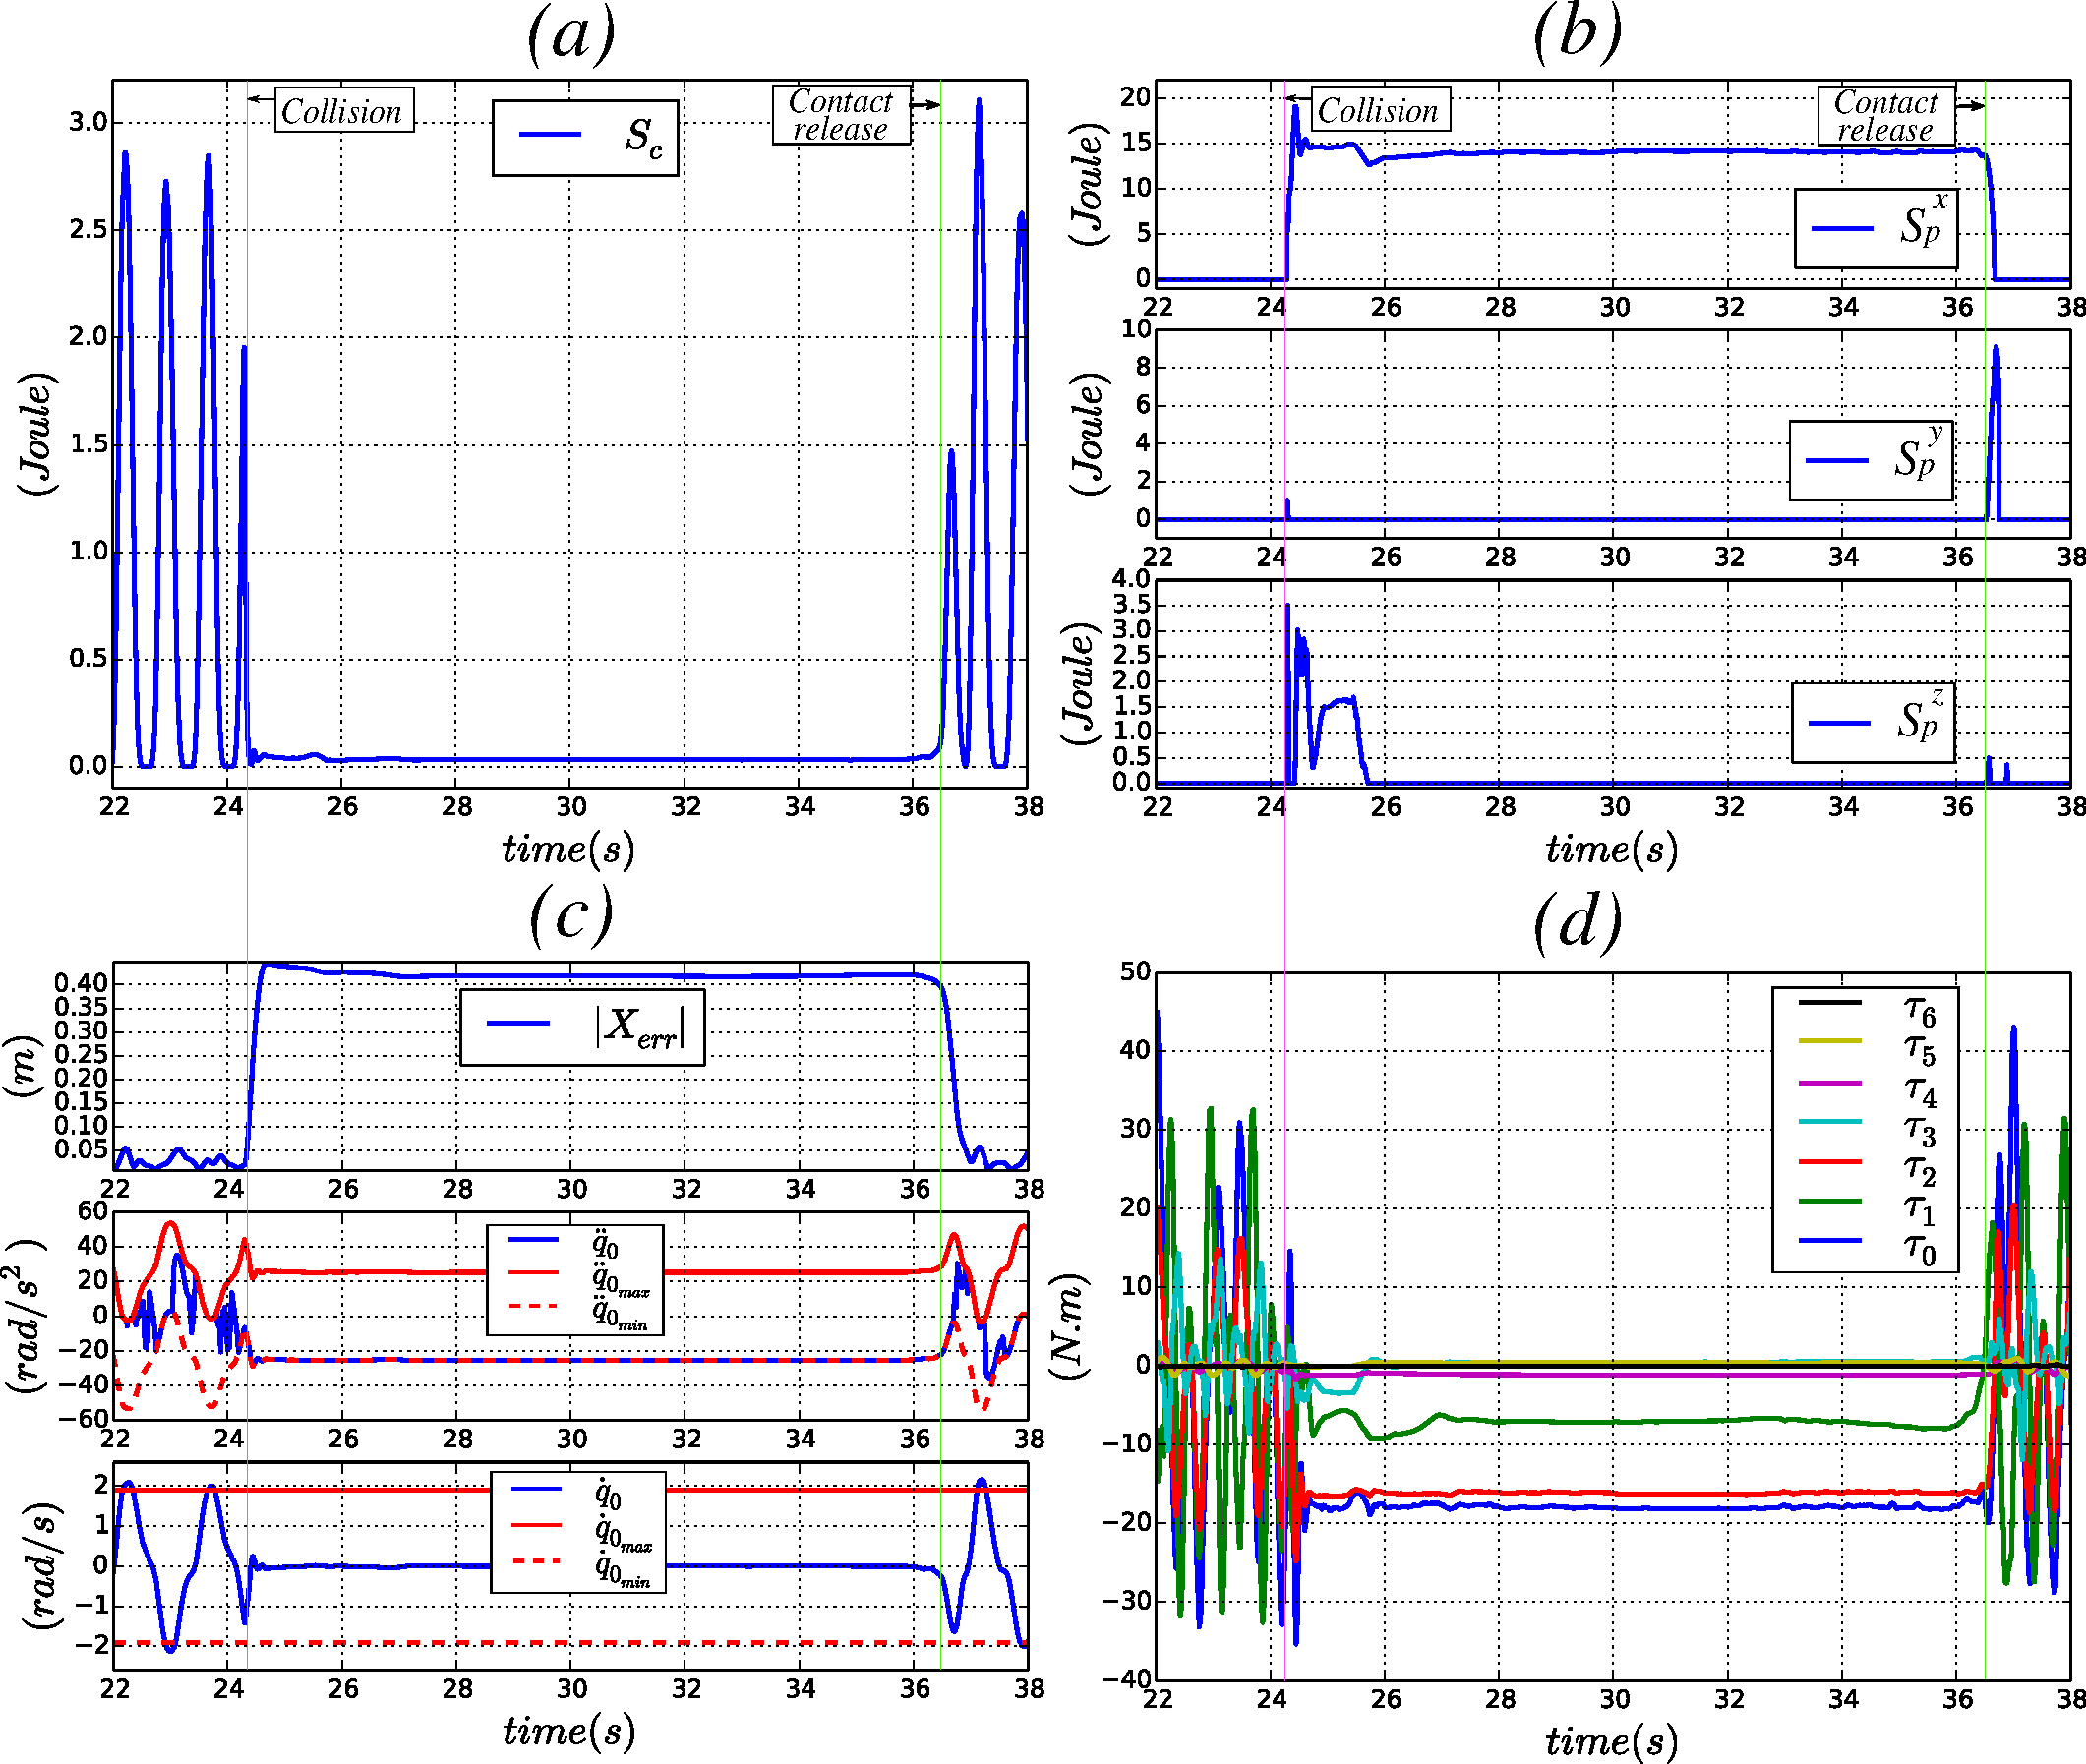
\includegraphics[width=0.84\linewidth]{figures/vel_track_woO_Ec_woEc1}
    \caption{(a) Kinetic energy of the robot's end-effector in the direction of the human operator; (b) Potential energy within the robot-human system during physical contact. (c) Top : position tracking error; Middle : constraint of the articular acceleration of the first joint; Bottom : articular velocity of the first joint. d) Articular torques}
    \label{fig:vel_track_woO_Ec_woEc1}
\end{figure}

The maximum position tracking error in the cartesian space (see (c) in Fig.~\ref{fig:vel_track_woO_Ec_woEc1}) is around $0.051~m$, this is mainly due to the activation of the the articular velocity constraint (\ref{eq:const_15}) on the robot's first joint. The maximum/minimum limits\footnote{The maximum/minimum limits on the articular velocity of the first joint are fixed in the QP at lower values than the real capacities of the robot.} on the articular velocity for the first joint are reached and violated. This is mainly caused by choosing $dt = 5 \cdot \delta t$ in (\ref{eq:const_15}). The reason for this choice and further explanations can be found in \cite{park1998enhanced}.
According to Fig.~\ref{fig:vel_track_woO_Ec_woEc1}, before the collision with the human operator\footnote{see video in \cite{kuka-url1}}, the maximum reached velocity of the robot end-effector in the cartesian space is about $2~m/s$ and the maximum kinetic energy in the direction of the human operator is $2.8~J$. At the collision instant, $2~J$ of kinetic energy are instantaneously dissipated to create the resulting impact force. 
 
After the establishment of physical contact, potential energy within the human-robot system increases to reach a maximum value of $14~J$ (see Fig.~\ref{fig:vel_track_woO_Ec_woEc1}~(b)). Consequently contact forces are created driving the blocked robot towards its desired position. The related torques can be seen in Fig.~\ref{fig:vel_track_woO_Ec_woEc1}~(d). Notice $\tau_0 \simeq -18~N.m$ and $\tau_2 = \simeq -16~N.m$. Once the physical contact released, the previously charged potential energy is transformed into kinetic energy as fast as possible and the robot goes back to its normal behaviour. 

%\subsection{Constraint on the kinetic energy and no constraint on the potential energy}
%In this scenario (see video) a constraint depending on the distance between the robot and the human operator is placed of the kinetic energy expressed at the robot end-effector in the direction of the human operator. After the collision and establishment of the physical contact, no constraint is placed on the potential energy generated within the human-robot system.



\subsection{Constraints on kinetic and potential energy}
In this scenario\footnote{see video in \cite{kuka-url2}}, the constraint (\ref{eq:Ec_constr_3}) depending on the distance between the robot and the human operator is placed on the kinetic energy expressed at the robot's end-effector in the direction of the human operator. After the establishment of physical contact, the constraint (\ref{eq:Ep_constr_4}) on the amount of potential energy allowed to be generated within the human-robot system is also activated.  
\begin{figure}[!ht]
    \centering
    \captionsetup{width=.84\linewidth}
	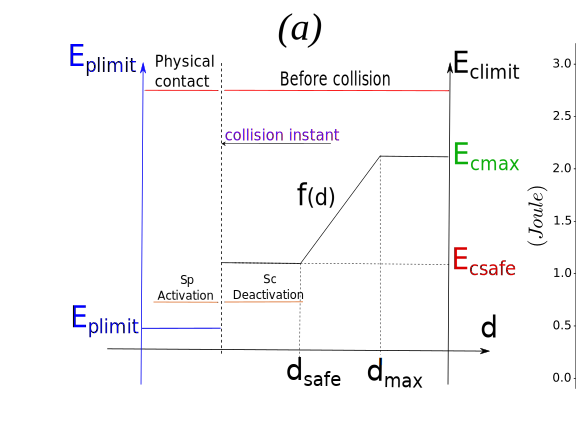
\includegraphics[width=0.84\linewidth]{figures/vel_track_woO_Ec_woEc2}
    \caption{(a) Evolution of the kinetic energy constraint depending on the distance d between the robot and the human operator. (b) Constrained Kinetic energy of the robot end-effector in the direction of the human operator; (c) Articular torques; (d) Potential energy within the human-robot system during physical contact.}
    \label{fig:vel_track_woO_Ec_woEc2}
\end{figure}
The controller parameters are chosen as following : $E_{safe} = 0.02~J$, $K = 0.4~N.m$, $d_{safe} = 0.3~m$ and $d_{max} = 7~m$. From the kinetic energy profile in Fig.~\ref{fig:vel_track_woO_Ec_woEc2}, the constraint on the kinetic energy of the robot is respected during the whole interaction's time. At the collision instant, comparing to the previous scenario, only $0.02~J$ of kinetic energy are dissipated; This results into a smaller impact force. 

After the establishment of physical contact, the constraint on the amount of potential energy allowed to be stored within the human-robot system is also respected at every time step (see Fig.~\ref{fig:vel_track_woO_Ec_woEc2}~(d)). In this case $E_{p_{safe}}^{x} = 0.0~J$, $E_{p_{safe}}^{y} = 0.0~J$ and $E_{p_{safe}}^{z} = 0.0~J$. This results in smaller contact forces.
The corresponding articular torques (see Fig.~\ref{fig:vel_track_woO_Ec_woEc2}~(c)) are much lower than during the contact phase of the previous scenario : $\tau_0 \simeq -4~N.m$ and $\tau_2 = \simeq -3~N.m$.  
%%%%%%%%%%%%%%%%%%%%%%%%%%%%%%%%%%%%%%%%%%%%%%%%%%%%%%%%%
%%%%%%%%%%%%%%%%%%%%%%%%%%%%%%%%%%%%%%%%%%%%%%%%%%%%%%%%%
                  %CONCLUSION%
%%%%%%%%%%%%%%%%%%%%%%%%%%%%%%%%%%%%%%%%%%%%%%%%%%%%%%%%%
%%%%%%%%%%%%%%%%%%%%%%%%%%%%%%%%%%%%%%%%%%%%%%%%%%%%%%%%%
\section{Conclusion and future work}
\vspace{-2 mm}
Using the presented control framework and the introduced energy based criteria, the robot has been proven capable to adapt to the human operator so
physical contact can be established without any damage. The impact force is reduced by constraining the kinetic energy of the robot and the contact force is modulated by constraining the amount of potential energy generated guring physical contact. In the presented experiments we have been able to ensure the respect at every time step of the constraints on potential and kinetic energy. The only way we have been able to implement these constraints is by controlling the system at a time step $\delta t = 15~ms$. Which gives the system sufficient time to brake and cope with these dynamic constraints. However, a time-step of $1~ms$ is still needed for better performances in the accomplishment of the trajectory tracking task.


\bibliographystyle{IEEEtran}
\bibliography{IEEEabrv,sampleTex}
\end{document}
